%% Slide
\subsection{What is XAS}

\begin{frame} \frametitle{X-ray Absorption Spectroscopy:  XAS, XAFS,  EXAFS and XANES.}

  \begin{cenpage}{125mm}

    X-ray Absorption Spectroscopy ({\Blue{XAS}}) is the modulation of
    the X-ray absorption coefficient at energies at and above an X-ray
    absorption edge.

    \vmm
    \begin{center}
      \begin{tabular}{ll}
        {\Blue{XAFS}} &  X-ray Absorption Fine-Structure Spectroscopy  (= XAS) \\
        {\Blue{XANES}} & X-ray Absorption Near-Edge Spectroscopy\\
        {\Blue{EXAFS}} & Extended X-ray Absorption Fine-Structure \\
      \end{tabular}
    \end{center}
    \vspace{1mm}

    These contain information about an element's chemical state (XANES) and
    local atomic environment (EXAFS).

    \end{cenpage}


    \begin{columns}[T]
      \begin{column}{62mm}
        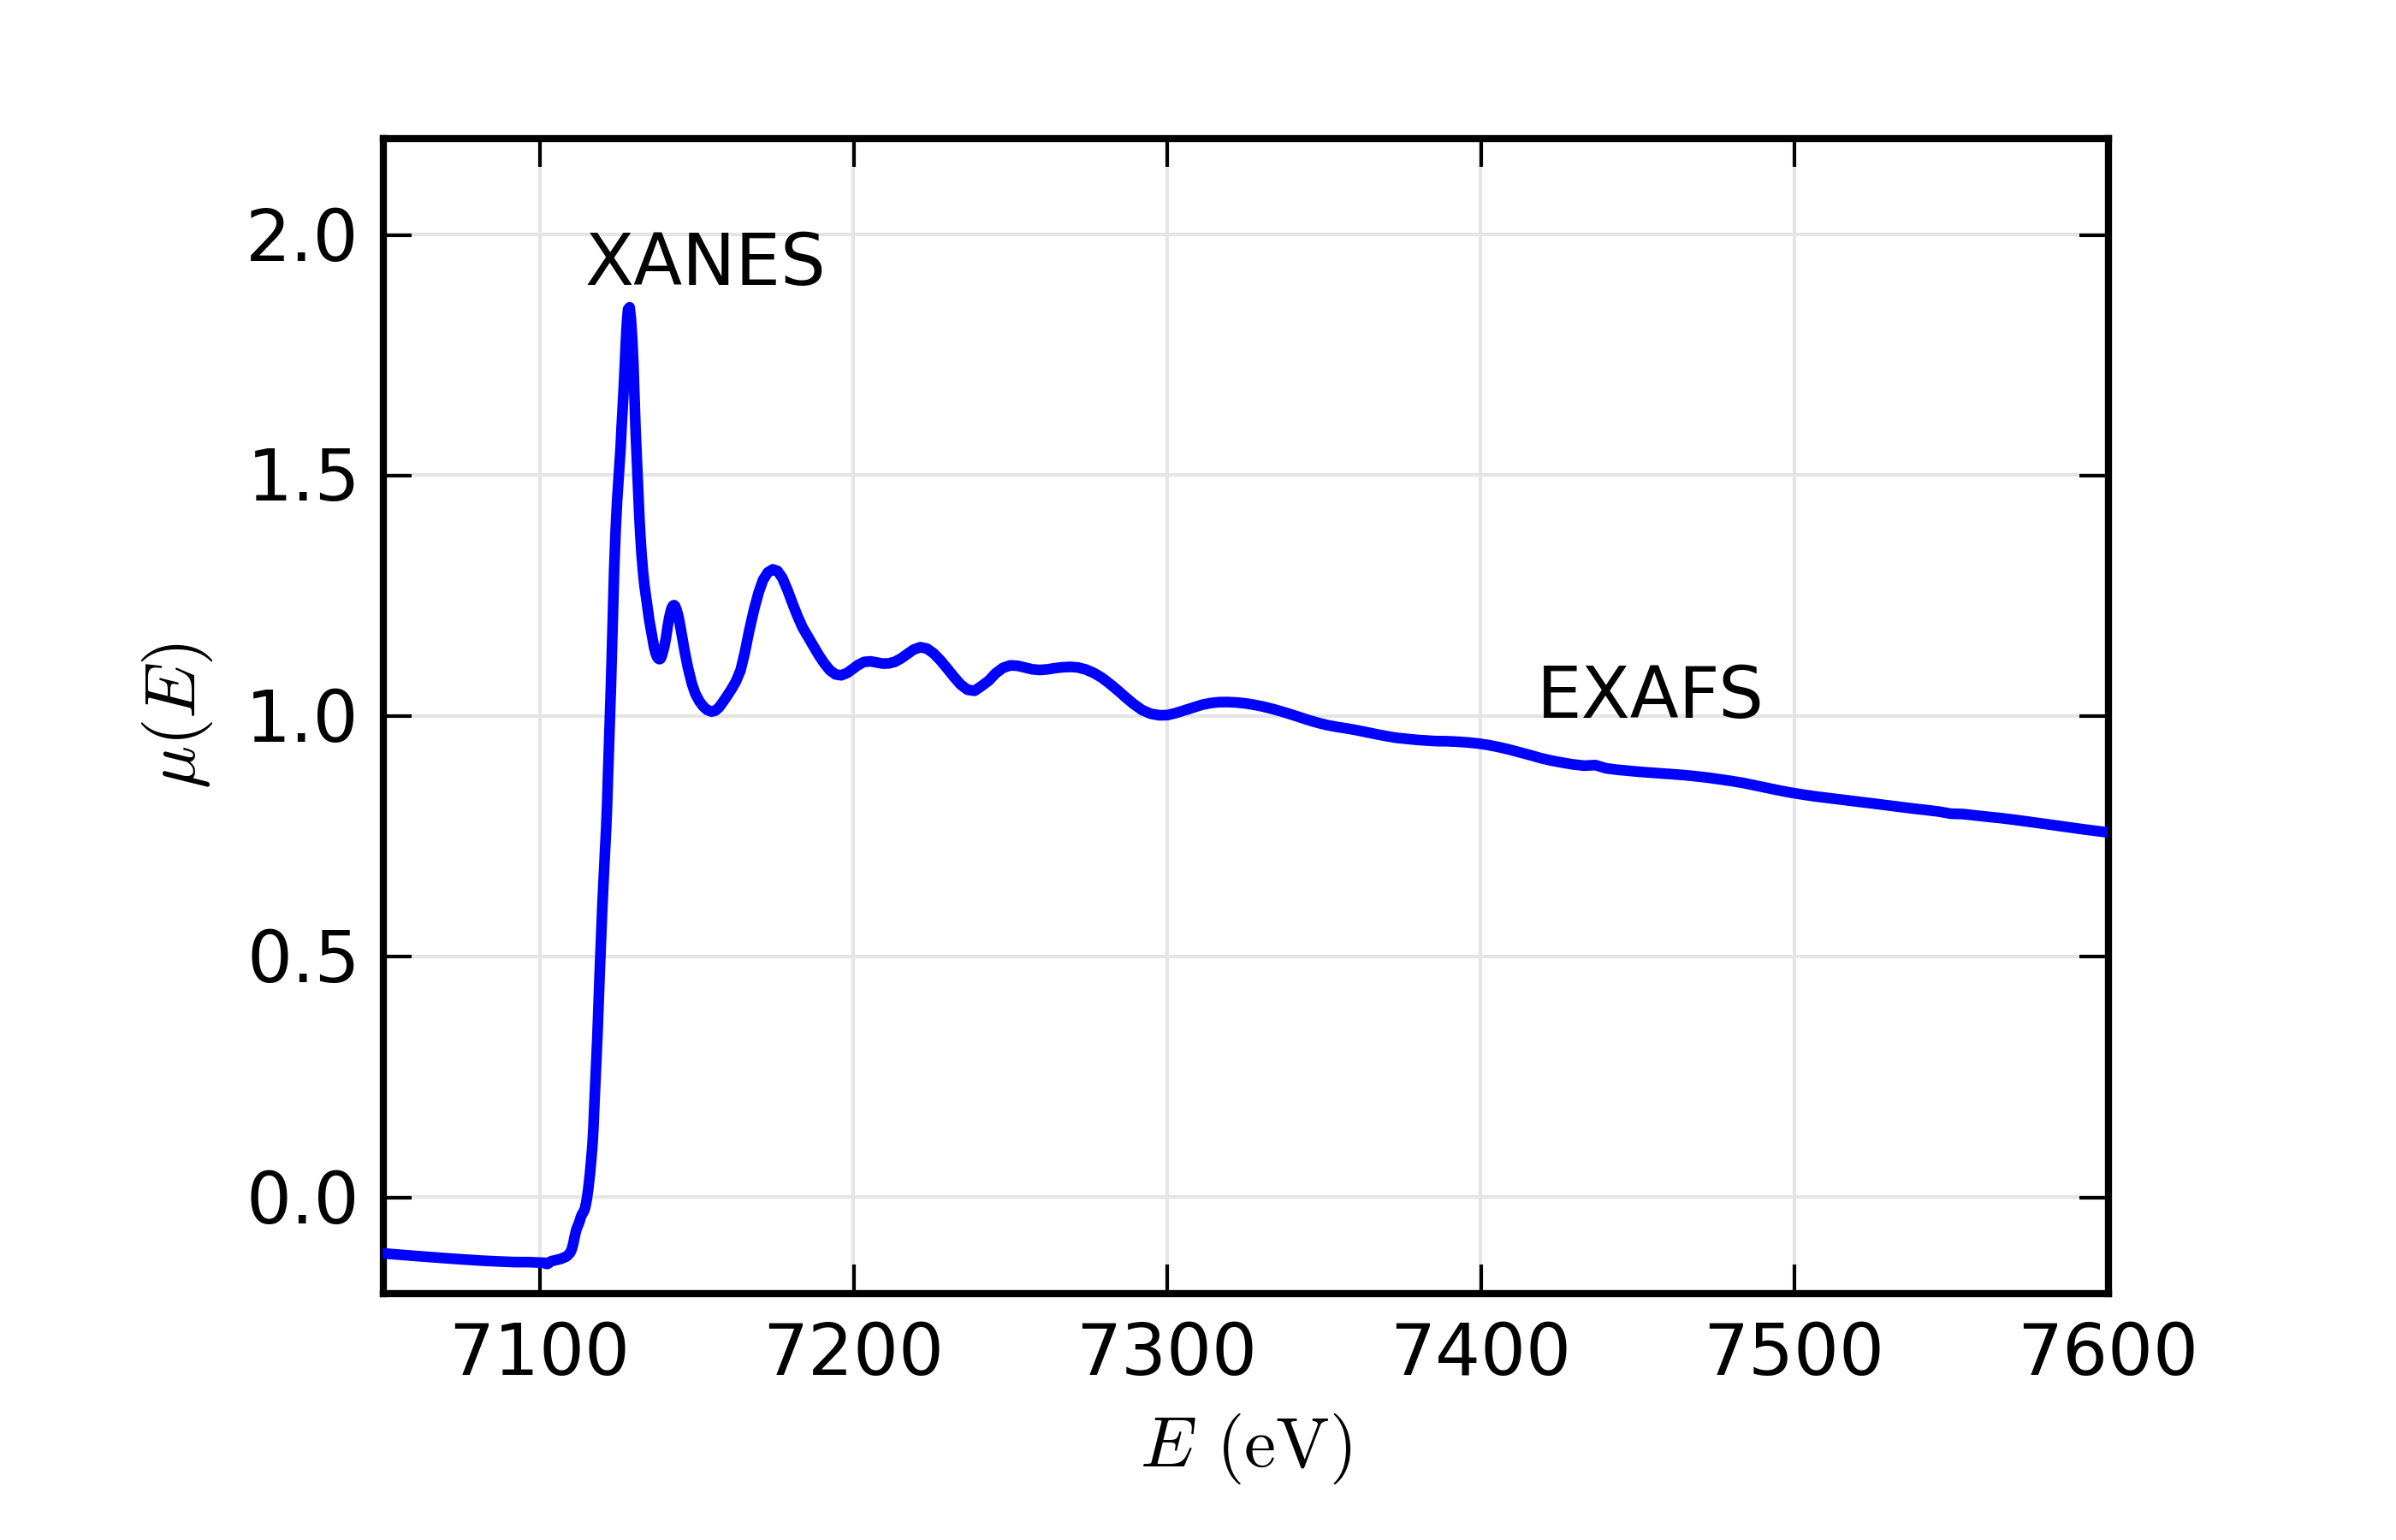
\includegraphics[width=58mm]{figs/rimg/mu_xanes_exafs}

        {\hspace{10mm} Fe {\slshape{K}}-edge XAFS for FeO}
      \end{column}
      \begin{column}{65mm}
        {\RedEmph{Main XAS Characteristics}}:
        \begin{itemize}
        \item local atomic coordination
        \item valence, oxidation state
        \item applies to any element ($Z > 2$) .
        \item works at low concentrations (ppm, $\mu$M)
        \item minimal sample requirements.
        \item independent of crystal  structure, isotope.
        \end{itemize}
      \end{column}
    \end{columns}

\vfill
\end{frame}
